% Chapter 5

\chapter{TR-069 Client} % Main chapter title

\label{Chapter5} % For referencing the chapter elsewhere, use \ref{Chapter5}

\lhead{Chapter 5. \emph{TR-069 Client}} % This is for the header on each page - perhaps a shortened title

\lstdefinestyle{DOS}
{
    backgroundcolor=\color{black},
    basicstyle=\scriptsize\color{white}\ttfamily
    numbers=none,
    numbersep=8pt,                   % how far the line-numbers are from the code
    numberstyle=\tiny\color{white}, % the style that is used for the line-numbers
    stepnumber=1                    % the step between two line-numbers. If it's 1, each line will be numbered
}
%----------------------------------------------------------------------------------------
\lstdefinestyle{C}
{
  morekeywords={export}
}
%----------------------------------------------------------------------------------------
TR-069 Client is implemented by Orange at 2008, but is a generic version for all potenial devices. The first part of my internship is to make TR-069 Client for Homelive Box. To be able to provide a generic TR-069 mudule which is easily portable on different devices, it satisfy the following points:

\begin{itemize}
  \item Written in ANSI C
  \item Small memory footprint
  \item Provide generic API to access device specific modules
  \item Provide Makefiles to build the binary
  \item Provide system traces on module activity
\end{itemize}

On a CPE, there are two modules that are mentioned all along this document and which are responsible of
the CWMP:
\begin{itemize}
  \item \textbf{TR-069 Agent}: This agent is responsible of the CWMP sessions. It initializes them with the inform message, realizes the ACS command(s) and execute some feedback command (notably after a firmware upgrade).
  \item \textbf{TR-069 Server}: This is a small HTTP server which listens of the WAN interface for an ACS solicitation (in TR-069, it is known as “connection request”). On a valid connection request, the TR-069 server contacts the TR-069 agent for starting a CWMP session with the ACS.
\end{itemize}
%----------------------------------------------------------------------------------------
\section{Architecture of TR-069 Client}
The TR069 Generic Agent is composed of several modules and interfaces. Some modules are generic and can be ported with no modification. Other modules are patform specific (specific libraries usage, specific device API to get/set values, ...) and must implement services declared into generic interfaces.

\begin{figure}[htbp]
	\centering
		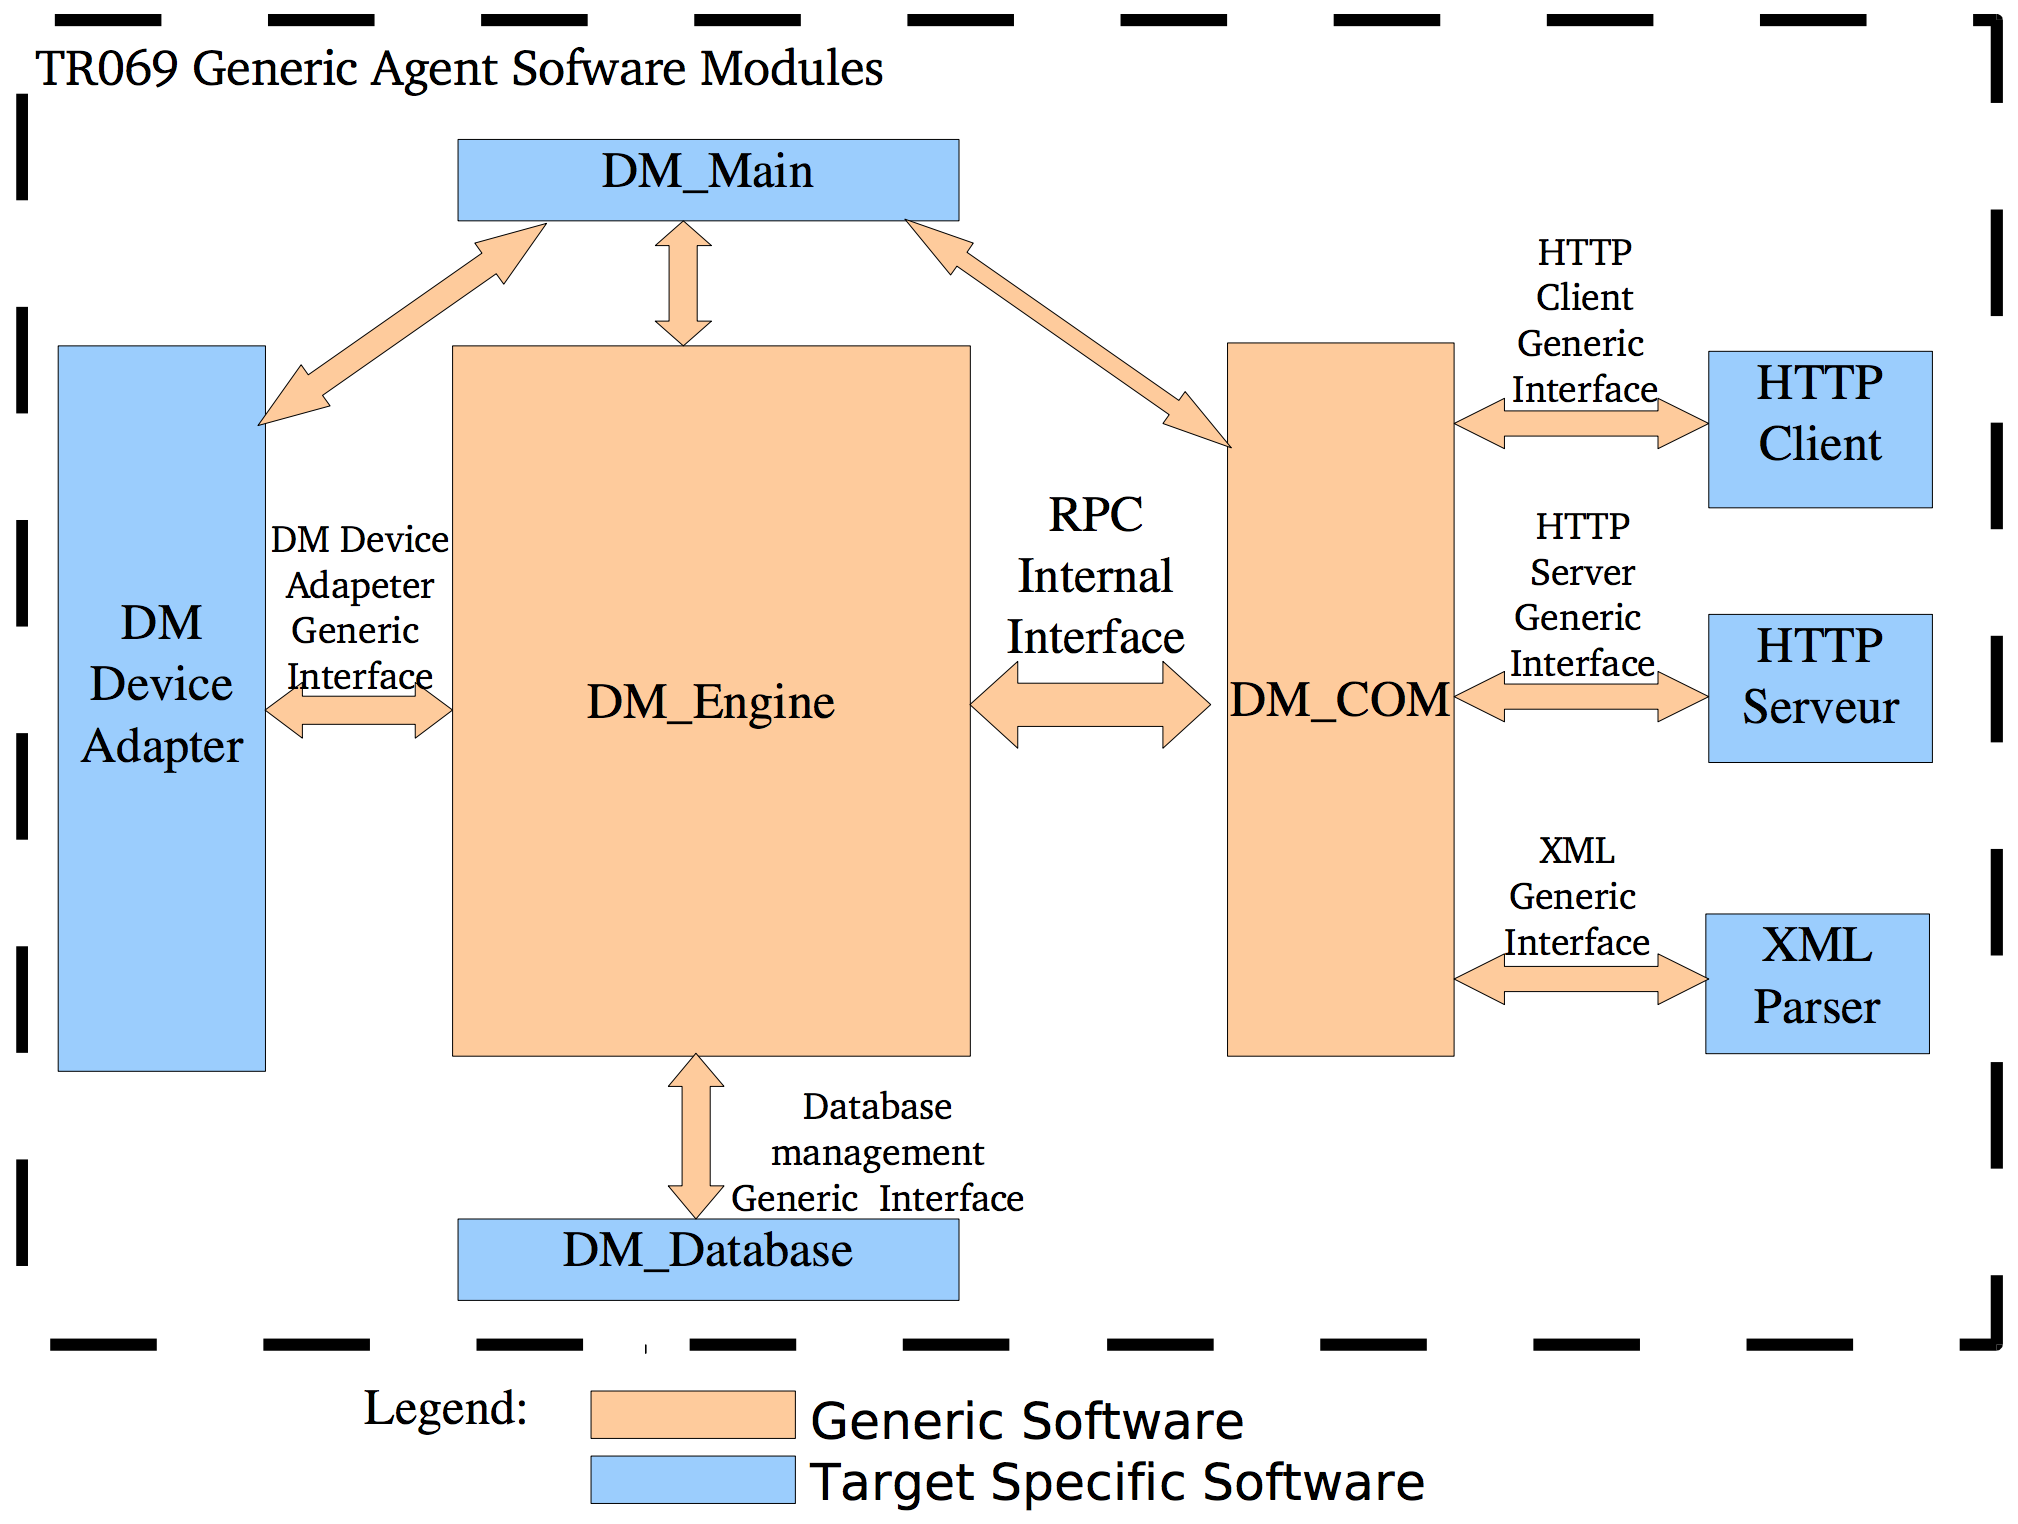
\includegraphics[width=12cm]{Figures/structuretr069.png}
	\caption[TR-069 Structure]{TR-069 Structure}
	\label{fig:tr069}
\end{figure}

For each module:
\begin{itemize}
  \item \textbf{DM\_ Engine} : In charge of the TR-069 logic,
  \item \textbf{DM\_ Com} : Handles the HTTP, SOAP and SSL Protocol with the ACS (Auto Configuration Server),
  \item \textbf{DM\_ DeviceAdapter} : Adaptation layer between the DM_Engine and the device system. It allows the implementation of the RPC commands (Get Parameter Value, Set Parameter Value, Reboot, Download, ...),
  \item \textbf{DM\_ Database} : Stores the data using an available storage solution on the device (or thanks to simple file storage),
  \item \textbf{HTTP Client} : Sets up / releases the HTTP connection with the ACS and sends / receives SOAP messages. The HTTP Client also handles SSL protocol,
  \item \textbf{HTTP SERVER} : Perform ACS Connection Request response,
  \item \textbf{XML Parser} : Decode / encode SOAP messages.
\end{itemize}

The figure below shows the file tree of the project, TR-069 Client defines all functions and APIs at each module. In consideration of easily ported to other devices, it put all target-related implementations in the folder \textit{dm\_target\_implementation}.

\begin{figure}[htbp]
	\centering
		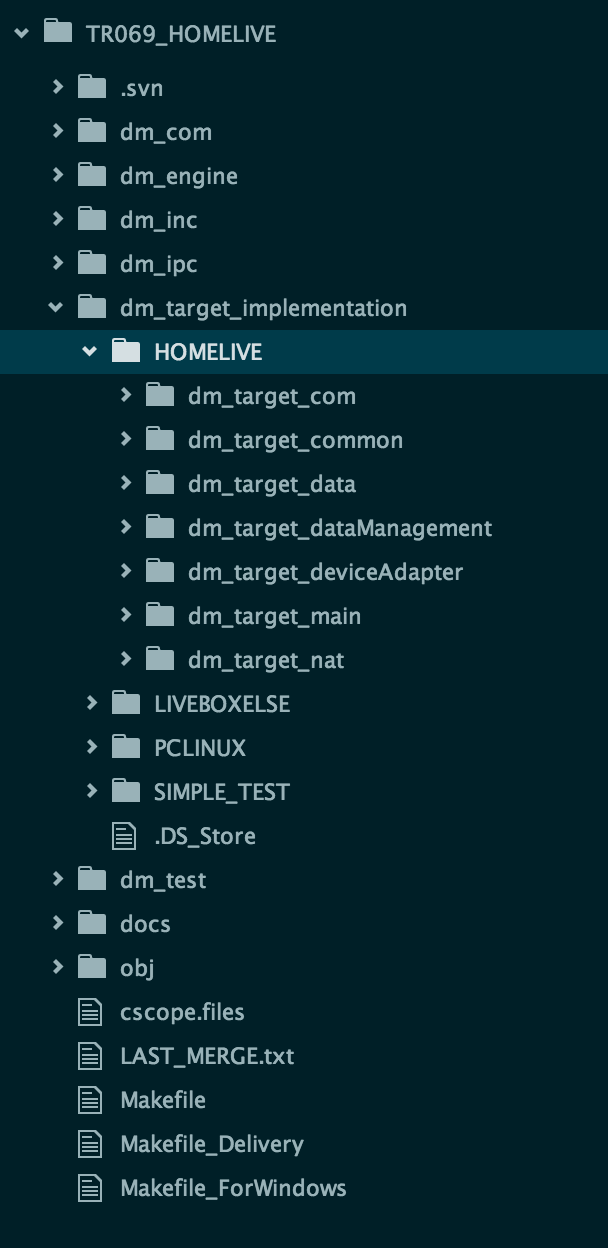
\includegraphics[width=8cm]{Figures/tr069_files.png}
	\caption[TR-069 File Tree Structure]{TR-069 File Tree Structure}
	\label{fig:tr069file}
\end{figure}

In the folder \textit{dm_taget_implementation}, different target has been defined, you can implement the APIs and Mudules for different devices, and you specifie the target to compile in compilation, like:

\begin{lstlisting}[style=DOS][language=bash]
  $ make Target=TargetName TRACE_LEVEL=7 DEBUG=Y
  $ make clean Target=TargetName
\end{lstlisting}

A csv file must be created for each new platform. This CSV file describes the data model parameters used by TR069 Agent and the default values for the TR069 specifics parameters. This target dependent CSV file is stored into \\\textit{dm\_target\_implementation/MYNEWDEVICE/dm\_dm\_target\_data/dm\_csv} directory.

The CSV file is only read during the first system start up (or after a factory reset) and is used to generate the TR069
database (i.e. parameters.data and parameters.data\~{} files)

%----------------------------------------------------------------------------------------

\section{Problems and Solutions}

When ported the TR-069 Client to Homelive, we have encountered serveral problems before it can perfectly running on Homelive Box.

%----------------------------------------------------------------------------------------

\subsection{IP Address Error}
The first problem is IP Address Error. At every start up of the TR-069 Client, the module will have to detect the IP address of the box, and use it to build connection between STUN server and CPE. But when executing, the TR-069 client can't detect the IP address, so I have located the code which are responsible for IP detection,

\begin{lstlisting}[mathescape]
    static const char* ETH_INTERFACE = "eth0";
    struct ifaddrs *myaddrs = NULL, *ifa = NULL;
    struct sockaddr_in *s4 = NULL;
    int  status;
    /* buf must be big enough for an IPv6 address (e.g. 3ffe:2fa0:1010:ca22:020a:95ff:fe8a:1cf8) */
    char buf[64];
    memset((void *) buf,  0x00, sizeof(buf));

    status = getifaddrs(&myaddrs);
    if (status == 0)
    {
       for (ifa = myaddrs; ifa != NULL; ifa = ifa->ifa_next)
       {
          if ( (ifa->ifa_addr != NULL)
             && ((ifa->ifa_flags & IFF_UP) != 0)
             && (ifa->ifa_addr->sa_family == AF_INET) )
          {
             s4 = (struct sockaddr_in *)(ifa->ifa_addr);
             if ( (inet_ntop(ifa->ifa_addr->sa_family, (void *)&(s4->sin_addr), buf, sizeof(buf)) != NULL)
                && (strcmp(ifa->ifa_name, ETH_INTERFACE)==0) )
             {
                ipAddress = strdup(buf);
                break;
             }
          }
       }
    }
\end{lstlisting}

In general, the first Internet address should be \textit{eth0}, but in Homelive Box, if you verify with command
\begin{lstlisting}[style=DOS][language=bash]
  $ ifconfig -a
\end{lstlisting}

The default Internet interface is "br-lan", which is specific in OpenWRT system, which is bridgeds Virtual Network Interface, used to make multiple virtual or physical network interfaces act as if they were just one network interface (quasi the opposite of VLANs).

So the solution is to change the macro definition of \textit{ETH\_INTERFACE} from \textit{``eth0''} to \textit{``br-lan''}. After the modification, the program can success finding the IP address.
%----------------------------------------------------------------------------------------
\subsection{STUN Initialisation}

When using the default data model provided, TR-069 Client can't build connection with STUN server. By looking into the log file, the problem aims to no STUN data model has been settled. The solution is to add the items which describe STUN parameters as follow:
\begin{lstlisting}[mathescape]
    ManagementServer.UDPConnectionRequestAddress;STRING;0;0;1;2;1;0;;0;0;0
    ManagementServer.UDPConnectionRequestAddressNotificationLimit;UINT;0;1;0;0;0;0;;0;0;0
    ManagementServer.STUNEnable;BOOLEAN;0;1;0;0;1;0;;1;0;0
    ManagementServer.STUNServerAddress;STRING;0;1;0;0;1;0;;161.105.161.211;0;0
    ManagementServer.STUNServerPort;INT;0;1;0;0;1;0;;3478;0;0
    ManagementServer.STUNUsername;STRING;0;1;0;0;0;0;;test;0;0
    ManagementServer.STUNPassword;STRING;0;1;0;0;0;0;;1234;0;0
    ManagementServer.STUNMaximumKeepAlivePeriod;INT;0;1;0;0;0;0;;400;0;0
    ManagementServer.STUNMinimumKeepAlivePeriod;UINT;0;1;0;0;0;0;;10;0;0
    ManagementServer.NATDetected;BOOLEAN;0;0;1;2;1;0;;0;0;0
\end{lstlisting}
%----------------------------------------------------------------------------------------
\subsection{Memory Alignement Error}
After the modifications above, everytime when running the TR-069 Client, after 2 seconds, the program crashs and report \textit{bus error}, a bus error is a fault raised by hardware, notifying an operating system (OS) that a process is trying to access memory that the CPU cannot physically address: an invalid address for the address bus, hence the name. In modern use on most architectures these are much rarer than segmentation faults, which occur primarily due to memory access violations: problems in the logical address or permissions.

Beacause the TR-069 is generated by cross-compiling, some platforms (in our case MIPS64) can only read or write ints from addresses that are an even multiple of 8 bytes, otherwise they segfault. Even the ones that can handle arbitrary alignments are slower dealing with unaligned data (they have to fetch twice to get both halves), so the compiler will often pad structures to align variables. Treating structures as a lump of data that can be sent to disk or across the network thus requires extra work to ensure a consistent representation.

In the source code, there are \textit{struct} defined like :
\begin{lstlisting}[mathescape]
    typedef struct _DM_ENG_Parameter
    {
    	bool writable; //1 byte
    	char* name;  // 4 bytes
      int minValue; // 4 bytes

      ....

      struct _DM_ENG_Parameter* next;
    } __attribute((packed)) DM_ENG_Parameter;
\end{lstlisting}


In a 32bits processor, the first three elements of the structure will be aligned like \fref{fig:side:a}. But when using the attribute (packed), the memory will become \fref{fig:side:b} to save the memory space.

\begin{figure}
\begin{minipage}[t]{0.5\linewidth}
\centering
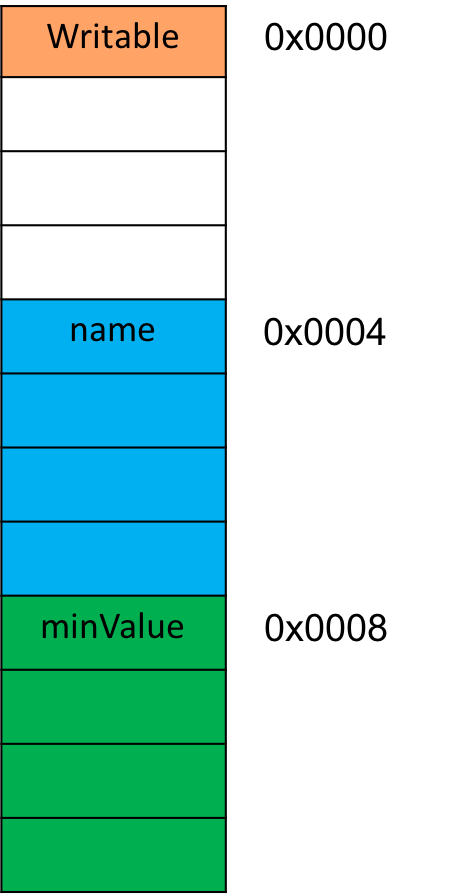
\includegraphics[width=4cm]{Figures/alignement1.png}
\caption{Memory Algnement under 32bits system}
\label{fig:side:a}
\end{minipage}%
\begin{minipage}[t]{0.5\linewidth}
\centering
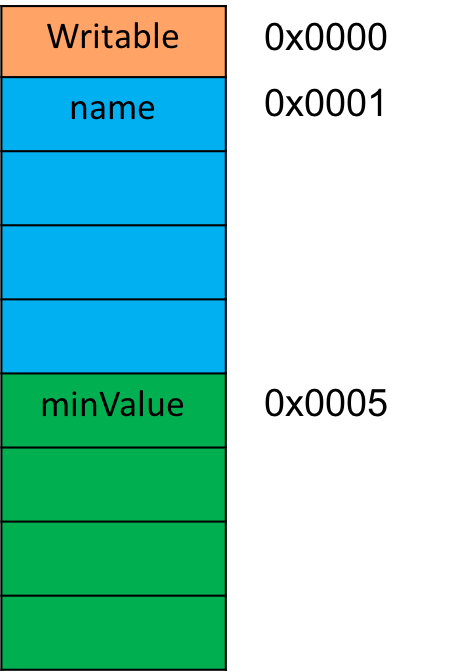
\includegraphics[width=4cm]{Figures/alignement2.png}
\caption{Memory Algnement under 32bits system with packed}
\label{fig:side:b}
\end{minipage}
\end{figure}


Under the Homelive architecture, it can only read data from address that is multiple of 4, so when the program tries to read value of name, the address is 0x0001 which is not an valid address, it reports the \textit{bus error}. To solve this bus error, the easiest way is to delete the attribute \textit{packed}, and then the compilator will automatique shift the address to meet the requirements.

%----------------------------------------------------------------------------------------
\section{RPC methods}
The next step is to verify and implemente all the RPC methods, after verification:
\begin{center}
  \begin{tabular}{@{} cc @{}}
    \toprule
    RPC Method & Result \\*
    \midrule
    Connection Request & Yes \\
    Get RPC Methods & Yes \\
    Set Parameter Values  & Yes\\
    Get Parameter Values  & Yes\\
    Set Parameter Attributes  & Yes\\
    Get Parameter Attributes  & Yes\\
    Get Parameter Names & Yes\\
    Add Object  & Yes\\
    Delete Object & Yes\\
    Reboot & No\\
    Downloaded  & Yes\\
    Factory Reset & Yes\\
    Schedule Inform & Yes\\
    Upload & Yes\\
    \bottomrule
  \end{tabular}
%	\caption[Homelive Box of Orange]{Homelive Box of Orange}
\end{center}

When we call \textit{reboot} from ACS, the TR-069 turns out only reboot the program but not the whole box. To repair this, after located the reboot function, we added one line at the end of the function to let the program call the box to reboot after 5 seconds (which is for the TR-069 to shutdown all the process).
\begin{lstlisting}[mathescape]
  /*Reboot system after 5 seconds*/
  system("(sleep 5 && reboot) &");
\end{lstlisting}
